%%%%%%%%%%%%%%%%%%%%%%%%%%%%%%%%%%%%%%%%%
% Arsclassica Article
% LaTeX Template
% Version 1.1 (10/6/14)
%
% This template has been downloaded from:
% http://www.LaTeXTemplates.com
%
% Original author:
% Lorenzo Pantieri (http://www.lorenzopantieri.net) with extensive modifications by:
% Vel (vel@latextemplates.com)
%
% License:
% CC BY-NC-SA 3.0 (http://creativecommons.org/licenses/by-nc-sa/3.0/)
%
%%%%%%%%%%%%%%%%%%%%%%%%%%%%%%%%%%%%%%%%%

%----------------------------------------------------------------------------------------
%	PACKAGES AND OTHER DOCUMENT CONFIGURATIONS
%----------------------------------------------------------------------------------------

\documentclass[
10pt, % Main document font size
a4paper, % Paper type, use 'letterpaper' for US Letter paper
oneside, % One page layout (no page indentation)
%twoside, % Two page layout (page indentation for binding and different headers)
headinclude,footinclude, % Extra spacing for the header and footer
BCOR5mm, % Binding correction
]{scrartcl}

%%%%%%%%%%%%%%%%%%%%%%%%%%%%%%%%%%%%%%%%%
% Arsclassica Article
% Structure Specification File
%
% This file has been downloaded from:
% http://www.LaTeXTemplates.com
%
% Original author:
% Lorenzo Pantieri (http://www.lorenzopantieri.net) with extensive modifications by:
% Vel (vel@latextemplates.com)
%
% License:
% CC BY-NC-SA 3.0 (http://creativecommons.org/licenses/by-nc-sa/3.0/)
%
%%%%%%%%%%%%%%%%%%%%%%%%%%%%%%%%%%%%%%%%%

%----------------------------------------------------------------------------------------
%	REQUIRED PACKAGES
%----------------------------------------------------------------------------------------

\usepackage[
nochapters, % Turn off chapters since this is an article        
beramono, % Use the Bera Mono font for monospaced text (\texttt)
eulermath,% Use the Euler font for mathematics
pdfspacing, % Makes use of pdftex’ letter spacing capabilities via the microtype package
dottedtoc % Dotted lines leading to the page numbers in the table of contents
]{classicthesis} % The layout is based on the Classic Thesis style

\usepackage{arsclassica} % Modifies the Classic Thesis package

\usepackage[T1]{fontenc} % Use 8-bit encoding that has 256 glyphs

\usepackage[utf8]{inputenc} % Required for including letters with accents

\usepackage{graphicx} % Required for including images
\graphicspath{{Figures/}} % Set the default folder for images

\usepackage{enumitem} % Required for manipulating the whitespace between and within lists

\usepackage{lipsum} % Used for inserting dummy 'Lorem ipsum' text into the template

\usepackage{subfig} % Required for creating figures with multiple parts (subfigures)

\usepackage{amsmath,amssymb,amsthm} % For including math equations, theorems, symbols, etc

\usepackage{varioref} % More descriptive referencing

%----------------------------------------------------------------------------------------
%	THEOREM STYLES
%---------------------------------------------------------------------------------------

\theoremstyle{definition} % Define theorem styles here based on the definition style (used for definitions and examples)
\newtheorem{definition}{Definition}

\theoremstyle{plain} % Define theorem styles here based on the plain style (used for theorems, lemmas, propositions)
\newtheorem{theorem}{Theorem}

\theoremstyle{remark} % Define theorem styles here based on the remark style (used for remarks and notes)

%----------------------------------------------------------------------------------------
%	HYPERLINKS
%---------------------------------------------------------------------------------------

\hypersetup{
%draft, % Uncomment to remove all links (useful for printing in black and white)
colorlinks=true, breaklinks=true, bookmarks=true,bookmarksnumbered,
urlcolor=webbrown, linkcolor=RoyalBlue, citecolor=webgreen, % Link colors
pdftitle={}, % PDF title
pdfauthor={\textcopyright}, % PDF Author
pdfsubject={}, % PDF Subject
pdfkeywords={}, % PDF Keywords
pdfcreator={pdfLaTeX}, % PDF Creator
pdfproducer={LaTeX with hyperref and ClassicThesis} % PDF producer
} % Include the structure.tex file which specified the document structure and layout

\hyphenation{Fortran hy-phen-ation} % Specify custom hyphenation points in words with dashes where you would like hyphenation to occur, or alternatively, don't put any dashes in a word to stop hyphenation altogether

%----------------------------------------------------------------------------------------
%	TITLE AND AUTHOR(S)
%----------------------------------------------------------------------------------------

\title{\normalfont\spacedallcaps{Der DES Algorithmus}} % The article title

\author{\spacedlowsmallcaps{Alexej Rotar \& Simon Sternsdorf\textsuperscript{1}}} % The article author(s) - author affiliations need to be specified in the AUTHOR AFFILIATIONS block

\date{30.3.2016} % An optional date to appear under the author(s)

%----------------------------------------------------------------------------------------
\usepackage{amssymb}
\usepackage{url}
\usepackage{parskip}
\begin{document}

%----------------------------------------------------------------------------------------
%	HEADERS
%----------------------------------------------------------------------------------------

\renewcommand{\sectionmark}[1]{\markright{\spacedlowsmallcaps{#1}}} % The header for all pages (oneside) or for even pages (twoside)
%\renewcommand{\subsectionmark}[1]{\markright{\thesubsection~#1}} % Uncomment when using the twoside option - this modifies the header on odd pages
\lehead{\mbox{\llap{\small\thepage\kern1em\color{halfgray} \vline}\color{halfgray}\hspace{0.5em}\rightmark\hfil}} % The header style

\pagestyle{scrheadings} % Enable the headers specified in this block

%----------------------------------------------------------------------------------------
%	TABLE OF CONTENTS & LISTS OF FIGURES AND TABLES
%----------------------------------------------------------------------------------------

\maketitle % Print the title/author/date block

\setcounter{tocdepth}{2} % Set the depth of the table of contents to show sections and subsections only

\tableofcontents % Print the table of contents

\listoffigures % Print the list of figures




%----------------------------------------------------------------------------------------
%	AUTHOR AFFILIATIONS
%----------------------------------------------------------------------------------------


%----------------------------------------------------------------------------------------

\newpage % Start the article content on the second page, remove this if you have a longer abstract that goes onto the second page

%----------------------------------------------------------------------------------------
%	INTRODUCTION
%----------------------------------------------------------------------------------------

\section{Einleitung}  
Verschlüsselung fand schon im alten Rom Anwendung. Einer der ersten und wohl auch bekanntesten Verschlüsselungsalgorithmen der Werlt, die sogeannte "Cäsar-Chiffre", findet man heutzutage in Popkultur um die ganze Welt. Es ist ein sehr einfaches symmetrisches Verfahren, bei dem das uns bekannte Alphabet zum Einsatz kommmt. Jeder Buchstabe wird durch einen anderen Buchstaben aus unserem Alphabet ersetzt, der um eine bestimmte Anzahl weiter hinten in der Reihenfolge steht. Das Ganze ist zyklisch und ergibt am Ende eine einfache Umwandlungstabelle. \footnote{\url{http://www.kryptowissen.de/caesar-chiffre.html} - 07.03.2016 13:50} Dieser Algorithmus ist heutzutage natürlich viel zu leicht zu knacken mit gerade einmal 25 verschiedenen Verschlüsselungsmöglichkeiten. Aber das Prinzip des symmetrischen Verschlüsselns mittels einer Chiffre ist uns bis heute erhalten geblieben. Der hier behandelte Algorithmus arbeitet im Grunde ganz ähnlich: Der DES Algorithmus.

\subsection{Geschichte} 
Der DES Algorithmus ist trotz seiner Sicherheitsprobleme immer noch einer der weltweit am weitesten verbreiteten Verschlüsselungsalgorithmen. Nicht umsonst heißt er Data Encryption Standart. Vor allem in dem Derivat "triple-DES" oder auch verkürzt "3DES" wird er noch eingesetzt und wird es wohl auch noch viele Jahre lang werden. Er wurde 1974 in Folge einer Ausschreibung des NBS, des National Bureau of Standars,  für einen sicheren Verschlüsselungsstandart zum Verschicken von Daten in den USA von IBM eingereicht. IBM beschäftigte damals unter anderem Horst Feistel, auf dessen Chiffren später genauer eingegangen wird. DES basiert grob auf dem schon zuvor entwickelten Algorithmus Luciver.\footnote{\url{http://page.math.tu-berlin.de/~kant/teaching/hess/krypto-ws2006/des.htm} - 07.03.2016 13:50} Die Verschlüsselung wurde 1976 nach Anpassungen der NSA, der National Security Agency, als allgemeiner Standart für verschlüsselte Datenverbindungen im Internet übernommen, und wurde vor allem von der Bankenindustrie und der US-Amerikanischen Regierung für die Kommunikation eingesetzt. \footnote{\url{http://page.math.tu-berlin.de/~kant/teaching/hess/krypto-ws2006/des.htm} - 07.03.2016 13:50}
 
\subsection{Kritik an Sicherheit}
Die Anpassungen der NSA sind sehr umstritten. So soll etwa der Sicherheitsgrad gesenkt worden sein durch Verkürzung der Schlüssellänge von 128 Bit auf 56 Bit und eventuell sogar die zur Verschlüsselung notwendigen Substitutions-Boxen von der NSA verändert worden sein.Man soll versucht haben sich eine Hintertür, einen sogenannten "backdoor" in den Algorithmus einzubauen. Da DES von Anfang an nur für den normalen Datenverkehr, aber nicht für Dokumente der höchsten Sicherheitsstufe eingesetzt wurde, ist es bis heute sehr umstritten wie sicher DES wirklich ist.\footnote{\url{http://www-lehre.informatik.uni-osnabrueck.de/~rspier/referat/internet/DES-Algorithmus.html} - 07.03.2016 13:50} Allerdings haben sich die meisten dieser Spekulationen nicht bestätigt.\footnote{Christian Karpfinger, Hubert Kiechle. Kryptologie. 1. Auflage. Seite 44. Vieweg+Teubner, 2010}
 
\section{Mathematische Grundlagen}
\subsection{Permutation und Expansion} 
Der DES-Algorithmus arbeitet mit sehr einfachen mathematischen Methoden. Der Schlüssel ist hierbei immer 64 Bit lang, wobei immer das letzte von 8 Bit als Korrektur-Bit verwendet wird, mit dem Speicher- und Übertragungsfehler ausgeglichen werden können.\footnote{Buchmann. Einführung in die Kryptologie. 4te, erweiterte Auflage. Seite 104. Springer-Verlag Berlin Heidelberg, 2008}  Dieser Schlüssel wird so zum Verschlüsseln auf die Nachricht angewandt, die jeweils in 64 Bit Blöcke unterteilt wird. Eine Permutation auf diese Bits entspricht einem Verschieben der Bits auf eine neue Position innerhalb des Blocks. Das Ganze wird gerne als Tabelle dargestellt, als sogenannte Permutations-Tabelle. 
\begin{figure}[h]
\centering
{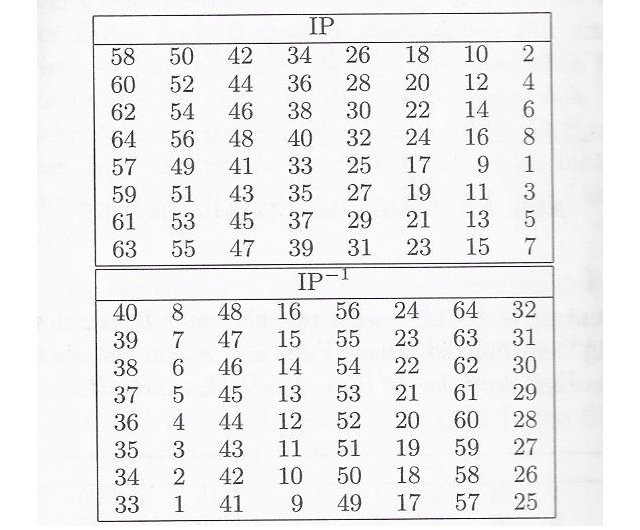
\includegraphics[width=.45\columnwidth]{PermutationsTabelle}} \quad
\caption[Eingangs-Permutations Tabelle]{Eingangs-Permuations Tabelle\footnotemark}
\label{fig:permutation}
\end{figure}
\footnotetext{Buchmann. Einführung in die Kryptologie. 4te, erweiterte Auflage. Seite 105. Springer-Verlag Berlin Heidelberg, 2008}
$\newline$
Jede Zahl beziffert genau die neue Position des Bits innerhalb des Permutatins-Blocks. So wird hier das erste Bit auf das 58te abgebildet, das zweite auf das 50te und so weiter. Nach dem selben Prizip wird dann die Expansion angewandt, allerdings ist dabei die Tabelle größer als der ursprüngliche Block. Das heißt hier werden manche Bits auf mehrere Stellen gesetzt.  
\subsection{Substitution}
Weiter wichtig sind zudem Substitutionen. Auf ihren Nutzen für die Sicherheit des Verfahrens wird später noch genauer eingegangen. Im Allgemeinen wird bei der Substitution ein Block an Bits durch einen anderen ersetzt. Dies geschieht wiederum durch Tabellen, wobei man hier beim DES auch von einer gleichzeitigen Kontraktion sprechen kann, da die Bitfolge verkürzt wird.
 \footnote{Buchmann. Einführung in die Kryptologie. 4te, erweiterte Auflage. Seite 107. Springer-Verlag Berlin Heidelberg, 2008} 

Expansion und Permutation sind lineare Abbildungen, wobei die Permutation eine Abbildung $\mathbb{Z}^{32}_2 \rightarrow \mathbb{Z}^{32}_2 $ und die Expansion eine Abbildung E: $ \mathbb{Z}^{32}_2 \rightarrow \mathbb{Z}^{48}_2 $sind.
Die Substitution ist eine nicht-lineare Abbildung.\footnote{Christian Karpfinger, Hubert Kiechle. Kryptologie. 1. Auflage. Seite 52. Vieweg+Teubner, 2010} 
\subsection{Kryptosysteme}
Wir verwenden in dieser Arbeit die Definition eines Kryptosystems wie folgt: 
Ein Kryptosystem ist ein Tupel(P, C, K, f, g) wobei P, C und K nicht leer sein dürfen. Hierbei ist: 
\begin{itemize} 
\item \textbf{P} die Klartextmenge, sprich der Text der verschlüsselt werden soll
\item \textbf{C} die Geheimtextmenge, sprich der verschlüsselte Text
\item \textbf{K} die Schlüsselmenge, also der Schlüssel der zum verschlüsseln der Klartextmenge zur Geheimtextmenge verwendet wurde
\item \textbf{f} die Verschlüsselungsfunktion, eine Abbildung $f: P \, x\,  K \rightarrow C$ , die aus der Klartextmenge die Geheimtextmenge bildet
\item \textbf{g} die Entschlüsselungsfunktion, eine Abbildung $g: C \, x \, K \rightarrow P$ , die aus der Geheimtextmenge die Klartextmenge bildet
\end{itemize}

Weiter muss gelten das $\forall k \in K : \exists k' \in K : g_{k'} \, o $ $ f_k = id_P $, was gleichbedeutent ist mit Injektivität und Surjektivität der Abbildung. Ohne diese Vorraussetzung wäre eine verschlüsselte Nachricht nicht mehr entschlüsselbar. Bei DES gilt $k' = k$. \footnote{Christian Karpfinger, Hubert Kiechle. Kryptologie. 1. Auflage. Seite 9. Vieweg+Teubner, 2010}
\section{Perfekte Sicherheit}
\subsection{Konzept}
Um zu verstehen wie sicher oder unsicher der DES-Algorithmus ist, braucht man das Konzept der perfekten Sicherheit. $\newline$ Hierbei gehen wir davon aus, dass der Angreifer über unendliche Rechenkapazitäten verfügt. Weiterhin haben wir ein Kryptosystem $ \pi = (P,C,K,f,g) $, das ein nach Kerckhoff's Prinzip sicheres Verschlüsselungsverfahren enthält, was heißt f und g sind allgemein bekannt.\footnote{\url{http://www.cits.rub.de/imperia/md/content/may/ws1516/krypto_i.pdf} - 09.03.2016 15:05}
Wir haben nun Wahrscheinlichkeits-Verteilungen Ws auf P,C und K, zudem sind $\textit{P}, \textit{C}$ und $\textit{K}$ die Zufallsvariablen für die Ws-Verteilungen. Nun ziehen wir ein $p \in P$ mit $Ws[\textit{P} = p]$ und analog für C und K. Die Wahrscheinlichkeit für $\textit{P} = p$ und $\textit{C} = c$ sollen dabei $> 0$ sein. Nun ist unser Kryptosystem und damit unser Verschlüsselungsverfahren sicher wenn der folgende Satz gilt: 
$\newline$
\newtheorem{satz}{Satz}

\begin{satz}
[Chiffretext-Verteilung] 

$$ Ws[ \textit{P} = p | \textit{C} = c] = Ws[\textit{P} = p] | \forall p \in P, c \in C $$  
\end{satz}
\begin{proof} 
 Annahme: $\pi$ sei perfekt sicher. Dann gilt nach Satz von Bayes: 
$$ \frac{Ws[ \textit{P} = p | \textit{C} = c] * Ws[\textit{P} = p]}{Ws[\textit{C} = c]} = Ws[ \textit{P} = p | \textit{C} = c] =  Ws[\textit{P} = p]$$

Daraus folgt $$Ws[ \textit{P} = p | \textit{C} = c] = Ws[\textit{C} = c] $$
Aus $Ws[ \textit{P} = p | \textit{C} = c] = Ws[\textit{C} = c]$ folgt mit dem Satz von Bayes:
 $$Ws[\textit{P} = p] = Ws[ \textit{P} = p | \textit{C} = c]$$
Damit ist nachgewiesen, dass $\pi$ perfekt sicher ist.
\end{proof}
Der für diesen Satz nötige Satz lautet wie folgt: 
$\newline$
\begin{satz}
[Satz von Bayes]
$\newline$
Für zwei Ereignisse A und B, wobei $B \neq 0 $ : 
$$ P_B (A) = \frac{P(A) * P_A (B)}{P(B)}$$ 
Hierbei bezeichnet $P_B (A) $ die Wahrscheinlichkeit des Ereignisses A unter Vorraussetzung des Eintretens von Bedingung B.
Equivalent für $P_A (B) $
$P(A) $ ist die sogenante Anfangswahrscheinlichkeit für das Ereignis A. Sie meint, dass das Ereignis A unabhängig zu betrachten ist. \footnote{\url{http://matheguru.com/stochastik/36-satz-von-bayes.html} - 25.03.2016 15:50} 
\end{satz}
\footnote{\url{http://www.mathebibel.de/satz-von-bayes} - 25.03.2016 14:20}
Ein Angreifer der sowohl die entschlüsselte Nachricht wie auch die verschlüsselte besitzt hat mit diesem System keine Vorteile.\footnote{\url{http://www.cits.rub.de/imperia/md/content/may/0910/ws0910/krypto1ws09/02_perfekt.pdf}-Seite 5 - 09.03.2016 15:30}
Man kann auch sagen p und c sind stochastisch unabhängig. 
Mit dem Satz der Chiffren-Verteilung kann man folgendes nachweisen:
\begin{satz}
[Ununterscheidbarkeit von Verschlüsselung]
Ein Verschlüsselungsverfahren $\pi$ ist perfekt sicher wenn gilt: 
$$p_0 , p_1 \in P, c \in C : Ws[ \textit{P} = p_0 | \textit{C} = c] =  Ws[ \textit{P} = p_1 | \textit{C} = c]$$
\end{satz}
\begin{proof}
Aus Satz 1 folgt für ein $\pi$ das perfekt sicher ist: 
$$Ws[ \textit{P} = p_0 | \textit{C} = c] = Ws[ \textit{C} = c]$$
$$ \exists c \in C : Ws[ \textit{C} = c] = Ws[ \textit{P} = p_1 | \textit{C} = c] $$
Sei $ p' \in P$ frei wählbar. Dann gilt: 
$$Ws[ \textit{C} = c] = \sum_{p \in P} Ws[ \textit{P} = p | \textit{C} = c] * Ws[ \textit{P} = p] $$
$$ = Ws[ \textit{P} = p' | \textit{C} = c] * \sum_{p\in P} Ws[ \textit{P} = p]$$
$$= Ws[ \textit{P} = p' | \textit{C} = c]$$
Insgesamt folgt daraus die perfekte Sicherheit von $\pi$ \footnote{\url{http://www.cits.rub.de/imperia/md/content/may/0910/ws0910/krypto1ws09/02_perfekt.pdf} - Seite 6 - 09.03.2016 16:20 }
\end{proof}
Man kann außerdem nachweisen, dass für das perfekte Verschlüsselungsverfahren gelten muss: 
\begin{satz}
[Minimale Größe des Schlüsselraumes]
Annahme: $\pi$ sei perfekt sicher. Dann gilt: $|K| \ge |P| $
\end{satz}
\begin{proof}
Beweis durch Widerspruch: 
Annahme: $|K| < |P| $
Für ein $c \in C$ definieren wir ein G(c) = {p | p = g(c,k) mit $k \in K$ }.
Es muss $|G(c)| \le |K|$ gelten, da ein Schlüssel k genau einen Klartext p liefert.  
Es gilt aber |K| < |P|. Daraus folgt das |G(c)| < |P|. Somit muss es ein $p \in P$ geben für das gilt: $Ws[\textit{P} = p | \textit{C} = c] = 0 < Ws[\textit{P} = p] $.
Das würde bedeuten, dass $\pi$ nicht perfekt sicher sein kann, da die Ws als > 0 definiert wurden. \footnote{\url{http://www.cits.rub.de/imperia/md/content/may/0910/ws0910/krypto1ws09/02_perfekt.pdf} - Seite 8 - 09.03.2016 16:20 }
\end{proof}
Mit dem Satz von Shannon können wir uns zudem noch die Verteilung der Schlüssel anschauen. 
\begin{satz} 
[Shannon]
Für ein Kryptosystem $\pi$ = (P,C,K,f,g) mit |P|=|C|=|K| gilt: $\pi$ ist perfekt sicher gdw : alle $k \in K$ werden durch f gleichverteilt gewählt mit einer Wahrscheinlichkeit von $ \frac{1}{|K|} $. Zudem gibt es für alle $p \in P, c \in C$ genau ein $k \in K $ sodass gilt: c = f(p,k).
\end{satz}
Hier beweisen wir zunächst die Gegenrichtung($\Leftarrow$): 
\begin{proof}
Wir können ein $ c \in C$ genau zu einem $p \in P$ entschlüsseln mit einem $k \in K $, bedeutet g(c,k) = p. Dies geschieht mit $Ws[\frac{1}{|K|}] $ gleichverteilt. Wir folgern: 
$$Ws[\textit{C} = c | \textit{P} = p] = \frac{1}{|K|}$$ für alle $p \in P$ 
Hieraus folgt mit Satz 2: 
$$Ws[\textit{C} = c | \textit{P} = p_0] = \frac{1}{|K|} = Ws[\textit{C} = c | \textit{P} = p_1]$$
Die Hinrichtung ($\Rightarrow$) folgt somit:
Widerspruchsbeweis:
Wir nehmen an: $\exists (p,c)$ mit $c \ne f(p,k)$ für alle $k \in K $
Deswegen gilt: $Ws[\textit{P} = p | \textit{C} = c] = 0 < Ws[\textit{P} = p]$. Dies steht im Widerspruch zu unserer Definition von einem perfekt sicherem System.
 
Nehmen wir anders herum an: $\exists (p,c)$ mit $c = f(p,k)$ für mehrere $k \in K (\ge 2) $.
Dann gilt: $\exists (p',c')$ mit $c' \ne f(p',k)$ für alle $k \in K $.
 
Dies erzeugt einen Widerspruch wie oben. 
Daraus folgern wir: Es gibt für jedes feste $p \in P, c \in C$ genau ein $k \in K$ für das gilt: f(p,k) = c. 
Im weiteren ergibt sich für alle p, p' : 
$Ws[\textit{K} = k_p] = Ws[\textit{C} = c | \textit{P} = p]$
$ = Ws[\textit{C} = c | \textit{P} = p'] = Ws[\textit{K} = k_p']$
$\rightarrow Ws[\textit{K} = k ] = \frac{1}{|K|}$ für alle $k \in K $\footnote{\url{http://www.cits.rub.de/imperia/md/content/may/0910/ws0910/krypto1ws09/02_perfekt.pdf} - Seite 9 - 09.03.2016 16:20 }
\end{proof}
$\newline$
Intuitiv bedeutet perfekte Sicherheit also: $\newline$
Der Schlüssel, der zur Verschlüsselung der Nachricht verwendet wird muss mindestens so lang sein wie die Nachricht selbst. Der Schlüssl muss zudem noch perfekt gleichverteilt von der Verschlüsselungsfunktion gewählt werden. Der Angreifer hat keinerlei Vorteile durch das Wissen um ein Klartext - verschlüsselter Text Paar. Das schließt auch sogenannte Meet-In-The-Middle Attacken aus, auf die später noch eingegangen wird. Mit all diesen nicht gerade leicht zu erfüllenden Bedingungen gibt es nicht viele Beispiele aus der Vergangenheit, von Verschlüsselungsverfahren die die Kriterien der perfekten Sicherheit erfüllten. 
\subsection{Vernam'sches One-Time-Pad}
Eines dieser wenigen Beispiel ist das Vernam'sche One-Time-Pad, eine 1918 von Gilbert Vernam entwickelte Verschlüsselungsmethode, die zum verschlüsseln des roten Telefons im Kalten Krieg zwischen dem US-Präsidenten und dem sowjetischen Generalsekretär genutzt wurde. Die Besonderheit ist, dass der Schlüssel genauso lang wie die zu verschlüsselnde Nachricht war. Zur Ver-und Entschlüsselung wurden Buchstaben nach einer Tabelle addiert. 

\begin{figure}[h]
\centering
{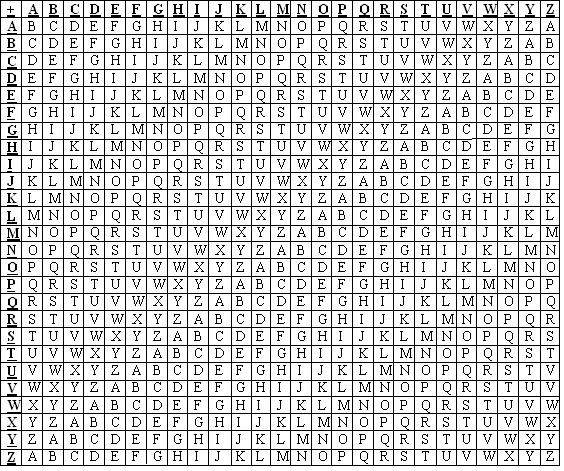
\includegraphics[width=.45\columnwidth]{OneTimePad}} \quad
\caption[One-Time Pad Tabelle]{One-Time Pad Tabelle\footnotemark}
\label{fig:Pad}
\end{figure}
\footnotetext{\url{http://www.mathe.tu-freiberg.de/~hebisch/Praktikum11-4/Seite2.html} - 09.03.2016 16:00}
Addiert wurde mit einer zufälligen Buchstabenfolge die beiden Seiten bekannt war.\footnote{\url{http://www.mathe.tu-freiberg.de/~hebisch/Praktikum11-4/Seite2.html} - 09.03.2016 - 16:00} Mathematisch wurde das One-Time-Pad definiert durch ein Kryptosystem $\pi = (P,C,K,f,g) $ wobei $ P=C=K=\{0,1\}^l $ für das gilt: 
$$ \exists k \in K, \exists p \in P : c \in C = f(p,k) = p \oplus k$$
$$ \exists k \in K, \exists c \in C : p \in P = g(c,k) = c \oplus k$$h
Annahme: Das One-Time-Pad ist ein perfekt sicheres Verfahren. 
\begin{proof}
Da $\textit{C} = \textit{P} \oplus \textit{K}$ gilt: 
$\forall p_0 , p_1 \in P und c \in C : Ws[\textit{C} = c | \textit{P} = p_0 ] = Ws[\textit{P} \oplus \textit{K} = p_0 ] = Ws [\textit{K} = p_0 \oplus c] $
$ = \frac{1}{2^l} = Ws[\textit{C} = c | \textit{P} = p_1 ]$
\end{proof}
Dies entspicht dem Satz über Ununterscheidbarkeit von Verschlüsselung.
Somit ist das One-Time-Pad perfekt sicher. \footnote{\url{http://www.cits.rub.de/imperia/md/content/may/0910/ws0910/krypto1ws09/02_perfekt.pdf} - Seite 7 - 09.03.2016 16:20 } $\newline$
Das Beispiel zeigt gut, wie wenig praktikabel eine Verschlüsselung mit perfekter Verschlüsselung im Alltag ist. Ein so langer Schlüssel macht nicht nur das Ver- und Entschlüsseln langsam, sondern fördert auch das Auftreten von Fehlern. Wenn beim One-Time-Pad die zufälligen Buchstabenfolgen nicht übereinstimmten oder etwa falsch gelesen wurden, konnten beide Seiten nicht mehr kommunizieren und es mussten neue Folgen ausgetauscht werden, was wiederum anfällig für Fehler und Angriffe von 3ten Parteien war. Somit kann das Ziel bei der Konstruktion eines Verschlüsselungsalgorithmus nie sein, ihn perfekt sicher zu machen, sondern nur sicher genug.
$\newline$
In der Realität haben die Angreifer auf eine Verschlüsselung nie unbegrenzte Resourcen zur Verfügung. Somit ist ein Schlüssel, der sehr viel kürzer als die Länge des Klartextes ist, oftmals ausreichend. 
Auch ist die Wahl eines Algorithmus, der die Schlüssel absolut gleichverteilt wählt, sehr schwierig und nur bei einem riesigem Schlüsselraum realistsisch. Ein solches Verschlüsselungsverfahren zu bauen und zu verwalten ist nicht praktisch. 
\section{Schluss}
\subsection{Kritik an DES} 
Schon recht früh nach Einführung des DES-Algorithmus als Standard-Verschlüsselung in vielen Bereichen des Öffenlichen Lebens kam Kritk auf. So wurde bereits früh, im Jahr 1975, vor der Möglichkeit eines Brute-Force Angriffs gewarnt, der aufgrund der recht kurzen Schlüssellänge gut möglich wäre. Im speziellen Martin Hellman und Whitfield Diffie, die Erfinder des Konzepts der Public-Key Verschlüsselung, warnten vor möglichen Angriffen von Regierungsorganisationen, im speziellen Geheimdienste. Diese hätten Zugriff auf die für damalige Verhältnisse recht hohe Rechenleistung.\footnote{\url{http://page.math.tu-berlin.de/~kant/teaching/hess/krypto-ws2006/des.htm} - 11.3.2016 - 17:20}  
\subsection{Brute-Force}
Ein Brute-Force-Angriff ist die einfachste und gewaltsamste Art eine Verschlüsselung zu knacken. Dabei wird von einem Computer systematisch jede Kombination aus Zahlen, Buchstaben und Sonderzeichen bis zu einer zuvor festgelegten Länge durchprobiert. Je kürzer dabei die Länge des verwendeten Schlüssels ist desto schneller ist das Verfahren. Zudem hängt es von der verwendeten Rechenpower des Angreifers ab. Ein höherer Einsatz von Rechenleistung erhöht die Geschwindigkeit der Suche.\footnote{\url{http://www.itwissen.info/definition/lexikon/Brute-Force-Angriff-brute-force-attack.html} - 11.03.2016 17:20} $\newline$
Moderne Verschlüsselungen setzen deswegen heutzutage auf Schlüssel, die sehr viel länger sind als die 56 Bit des DES-Algorithmus. Der weit verbreitete Verschlüsselungsalgorithmus AES setzt auf Schlüssellängen bis zu 256 Bit. \footnote{\url{https://www.boxcryptor.com/de/verschl} - 11.03.2016 - 17:30}
\subsection{Der DES-Cracker} 
Im Jahr 1998 gelang es schließlich der Electronic Frontier Foundation, eine Organisation die sich für digitale Grundrechte und Privatssphäre einsetzt, mithilfe einer selbst gebauten "Crackers" den DES-Algorithmus mittels Brute-Force zu knacken. Die Maschine kostete nur 250.000 Dollar und benötigte nur 3 Tage um diese Aufgabe zu bewerkstelligen. Die EFF wollte damit der Öffentlichkeit aufzeigen, wie leicht der immer noch in weiten Teilen der Industrie eingesetzte Verschlüsselungsalgorithmus zu knacken war.
\begin{figure}[tb]
\centering
\subfloat[Der verwendete Cracker-Chip.]{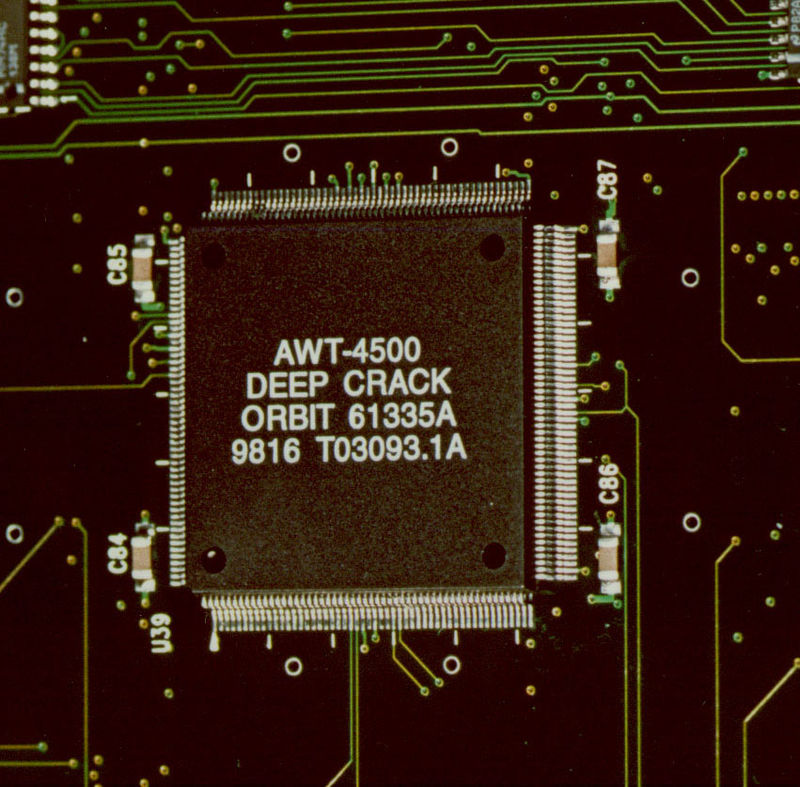
\includegraphics[width=.45\columnwidth]{Chip300}} \quad
\subfloat[Ein Chip-Board]{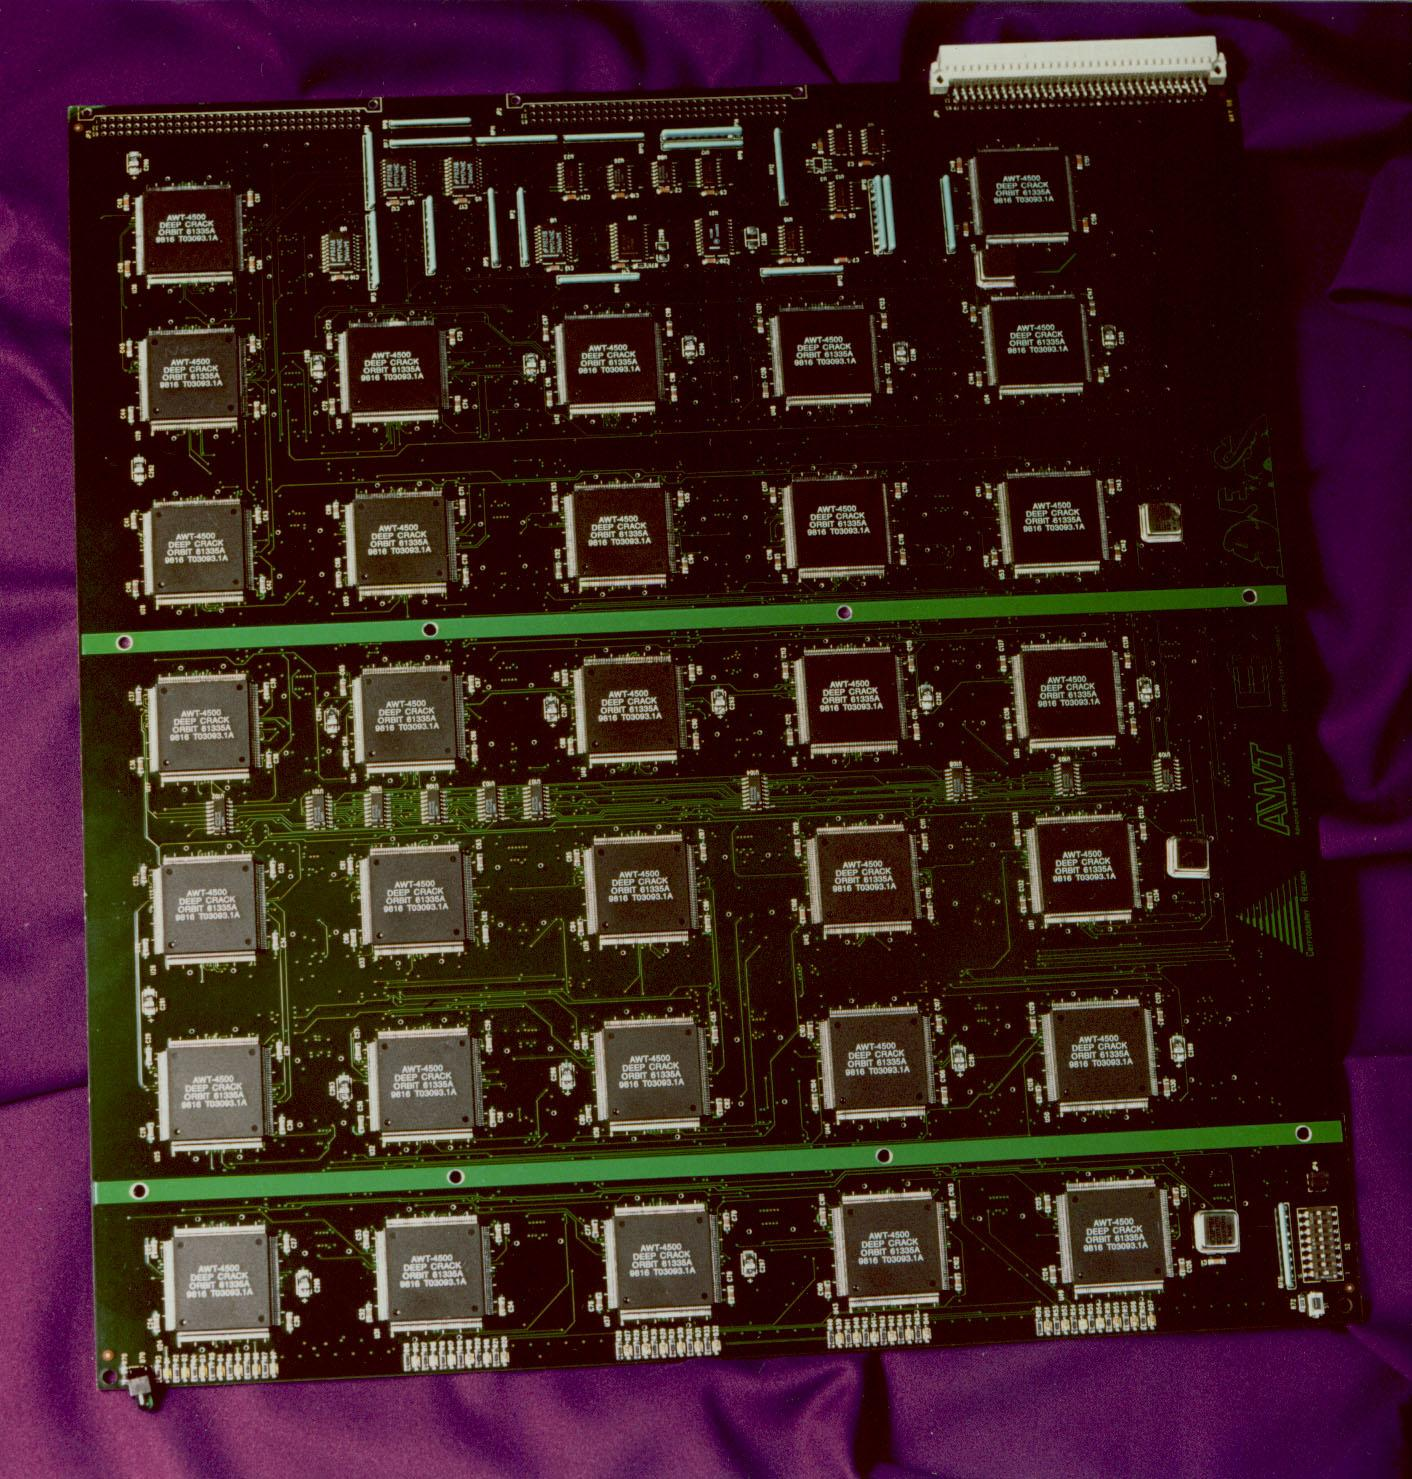
\includegraphics[width=.45\columnwidth]{board300}\label{fig:Chip}} \\
\caption[DES-Cracker.]{DES-Cracker Chip \footnotemark}
\label{fig:ChipBoard}
\end{figure}
\footnotetext{\url{https://w2.eff.org/Privacy/Crypto/Crypto_misc/DESCracker/} - 12.03.2016 - 15:20}
1999 gelang es mit dem DES-Cracker und einem weltweitem Computernetzwerk namens Distributed.Net eine DES-verschlüsselte Nachricht in nur 22 Stunden zu knacken. Die Computer schafften es zusammen auf eine Geschwindigkeit von 245 Millarden Schlüsseltests pro Sekunde. Das ganze geschah im Rahmen eines Wettbewerbs, um die von der US-Regierung immer noch bestehende Behauptung zu widerlegen, dass es Jahre brauchen würde und Rechenleistung im Wert von mehreren Millionen Dollar um eine DES-Nachricht mittels Brute-Force zu entschlüsseln. \footnote{\url{https://w2.eff.org/Privacy/Crypto/Crypto_misc/DESCracker/} - 12.03.2016 15:20}
\subsection{Entwickelte Alternativen} 
Die EFF schlug schon 1994 dem X9 Kommittee, das für die Empfehlung von neuen Verschlüsselungsalgorithmen verantwortlich war als Alternative triple-DES oder kurz 3DES vor. Damit stellten sie sich klar gegen die NSA und deren Vorschlag eines speziellen Verschlüsselungschips namens Clipper, der einen eingebauten "Backdoor" enthielt, um so der NSA Zugriff auf verschlüsselte Kommunikation zu geben. Ein Backdoor ist eine Hintertür in einem eigentlich als sicher geltendem System. In der Öffentlichkeit nichts von dieser Sicherheitslücke bekannt und sie wird nur von bestimmten Organisationen genutzt. Dabei wurde eine Backdoor im Gegensatz zu einem Exploit durch einen Programmfehler speziell beim Entwerfen des Programms eingebaut.\footnote{\url{http://www.itwissen.info/definition/lexikon/Backdoor-backdoor.html} - 12.03.2016 - 15:40} 
Die EFF schlug dabei 3DES aus den folgenden Gründen vor: 
\begin{itemize}
\item Grundsätzlich ist DES, auf dem 3DES basiert ein kryptologisch sicherer Algorithmus
\item Es eliminiert (für die damalige Zeit) die Möglichkeit einer Brute-Force-Attacke durch den viel längeren Schlüssel, der verwendet wird. Die Schlüssellänge wird zu DES verdoppelt.
\item Es ist leicht in bereits vorhandene Systeme für  DES zu integrieren
\end{itemize} 
\footnote{\url{https://www.eff.org/de/effector/7/14} - 12.03.2016 15:40}
\subsection{Ungeeignete Alternative: 2DES}
Da man mit 3DES die Schlüssellänge nur verdoppelt kann man sich fragen, warum man nicht einfach nur 2DES verwendet. Hierbei würde man mit 2 DES Schlüsseln einen Klartext zunächst mit dem 1ten Schlüssel und danach diesen verschlüsselten Text mit dem 2ten Schlüssel verschlüsseln. Da DES keine Gruppe ist würde dies tatsächlich nicht nur einem neuen Schlüssel entsprechen. Allerdings ist dieses Verschlüsselungsverfahren anfällig für die sogenannte Meet-in-the-middle Attacke. \footnote{\url{http://www.nku.edu/~christensen/3DES.pdf} - 25.03.2016 - 14:30} 
Die Meet-in-the-middle Attacke kann nur bei einem Verschlüsselungsalgorithmus mit einem sogenannten Intermediate State funktionieren. Eine kleine Darstellung einer Meet-in-the-Middle Attacke: 
$\newline$
\begin{figure}[h]
\centering
{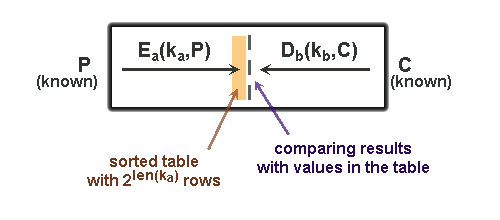
\includegraphics[width=.60\columnwidth]{attack_mitm_simple_eng}} \quad
\caption[Meet-In-The-Middle]{Darstellung einer Meet-In-The-Middle Attacke\footnotemark}
\label{fig:Pad}
\end{figure}
\footnotetext{\url{http://www.crypto-it.net/eng/attacks/meet_in_the_middle.html} - 28.03.2016 13:00}
$\newline$
Wir brauchen dabei einen Klartext P und den dazugehörigen verschlüsselten Text C. Wir haben nun also: $$ P \rightarrow f(P,k_1) \rightarrow f(f(P,k_1), k_2) \rightarrow C $$
Der Trick ist nun den Zustand $ f(P,k_1)$ zu erreichen. Dabei wird zuerst ganz klassisch mit Brute-Force der Klartext P mit allen möglichen Schlüsseln ($2^{56} $ Bit) verschlüsselt und die Resultate gespeichert. Danach macht man das gleiche mit C und der Entschlüsselungsfunktion.

Es gilt also: $ P \rightarrow f(P,k_1) = d(C,k_2) \leftarrow C $

 Man vergleicht immer mit dem Resultat der Verschlüsselung von P. Es kann dabei mehrere Paare geben die zusammen passen, aber endlich viele. Diese kann man dann ausprobieren ob sie auch bei anderen verschlüsselten Texten funktionieren um so die richtigen 2 Schlüssel herauszufinden. \footnote{\url{http://www.crypto-it.net/eng/attacks/meet_in_the_middle.html} - 25.03.2016 14:50} 

Größter limitierender Faktor war damals noch der hohe Speicherplatzverbrauch. Man brauchte die Kapazität die gesamten Intermediate Texte zu speichern. Das ist heutzutage kein Hindernis mehr. \footnote{\url{http://internetofthingsagenda.techtarget.com/definition/meet-in-the-middle-attack} - 25.03.2016 15:20}

Wenn man das Verfahren in 2 oder mehr einfachere Verfahren aufteilen kann, so ist es möglich eine sogeannte "mehrdimensionale MitM Attacke" durchzuführen. Dies  ist vor allem bei Blockchiffren ein Problem, die auf kleinen Datenblöcken mit sehr großen Schlüsseln agieren. Die Schlüssel werden hierbei effektiv aufgeteilt. 

$\newline$
\begin{figure}[h]
\centering
{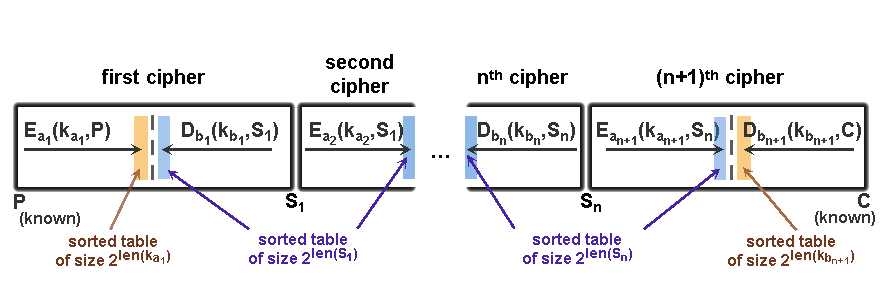
\includegraphics[width=.95\columnwidth]{attack_mitm_nd_eng}} \quad
\caption[mehrdimensionale MitM]{Darstellung einer mehrdimenionalen MitM Attacke\footnotemark}
\label{fig:Pad}
\end{figure}
\footnotetext{\url{http://www.crypto-it.net/eng/attacks/meet_in_the_middle.html} - 28.03.2016 13:10}
$\newline$

Schlussendlich bekommt man trotz der 2 verwendeten Schlüssel bei 2DES nicht eine resultierende Schlüssellänge von $2^{112} $ Bit, statdessen braucht man mit Brute-Force nur doppelt so lange um die Nachricht zu entschlüsseln, sollte man im Besitz eines Klartext- verschlüsselter Text Paares sein. Das enspricht $2^{57}$ Bit. Damit war 2DES nicht zukunftstauglich und wurde nicht in Betracht gezogen als Alternative für DES. \footnote{\url{http://www.nku.edu/~christensen/3DES.pdf} - 25.03.2016 15:00} 



\subsection{triple-DES}
3DES wurde im Standart X9.52 festgehalten und wurde zur neuen empfohlenen Verschlüsselungsmethode in der FIPS, der Federal Information Processing Standard. Dieser regelt die Standards, die Firmen erfüllen müssen um Verträge mit der US-Regierung zu schließen. Dies trug maßgeblich zu Verbreitung des 3DES in viele mit der Regierung zusammenhängenden Wirtschaftszweige bei. Zugleich wurde Single-DES oder DES nur noch für wenige, speziell zugelassene "legacy systems" erlaubt. Das sind Systeme die zu alt und groß waren, und die eher intern genutzt wurden. $\newline$
Zudem wurde die langsame Umstellung auf AES empfohlen, da dieser auch von der NSA speziell authorisiert war. Zunächst wollte man aber die hardwarebasierten DES-Systeme weiter nutzen, deswegen war 3DES ein logischer Schritt.\footnote{\url{http://csrc.nist.gov/publications/fips/fips46-3/fips46-3.pdf} - 12.03.2016 16:50} 
3DES basiert auf dem DES Algorithmus. Um etwas mit 3DES zu verschlüsseln nimmt man 2 DES Schlüssel mit jeweils 56 Bit und wendet sie wie folgt an: 
\begin{itemize}
\item Verschlüssele den Klartext mit dem ersten Schlüssel
\item Entschlüssle die Nachricht mit dem zweiten Schlüssel
\item Verschlüssle die Nachricht nochmal mit dem ersten Schlüssel
\end{itemize}
Diese besondere Anrt der Anwendug der 2 Schlüssel bedeutet eine Verlängerung des insgesamten Schlüssel auf 112 Bit. Dadurch ist er sehr viel schwerer mit Brute-Force zu knacken.\footnote{\url{http://page.math.tu-berlin.de/~kant/teaching/hess/krypto-ws2006/des.htm} - 12.03.2016 16:20}  
Es hat keinerlei Auswirkungen auf die Sicherheit des Verfahrens ob man in Schritt 2 und 3 ver-oder entschlüsselt. Aber in der oben genannten Reihenfolge ist es üblich. Man kann nur nicht immer den gleichen Schlüssel benutzen.\footnote{\url{http://www.itwissen.info/definition/lexikon/triple-DES-3DES-Dreifach-DES.html} - 12.03.2016 16:30} 

Ein Nachteil von 3DES im Gegensatz zu anderen Verschlüsselungsverfahren ist seine Performanz. Da auf Hardwareverschlüsselung optimiert, ist die dreimalige Anwendung des DES-Algorithmus in Software form deutlich langsamer als von vergleichbaren Algorithmen mit ähnlich hoher Sicherheit. Deswegen ist 3DES im Privatgebrauch auch kaum verbreitet. Hier hat sich vor allem AES durchgesetzt wegen seiner sehr reduzierten Codebasis.\footnote{\url{http://www.netplanet.org/kryptografie/verfahren.shtml} - 12.03.2016 16:30}

  


































%----------------------------------------------------------------------------------------
%	BIBLIOGRAPHY
%----------------------------------------------------------------------------------------

\renewcommand{\refname}{\spacedlowsmallcaps{References}} % For modifying the bibliography heading

\bibliographystyle{unsrt}

\bibliography{sample.bib} % The file containing the bibliography

%----------------------------------------------------------------------------------------

\end{document}